\documentclass[12pt]{article}
\usepackage[utf8]{inputenc}
\usepackage{amsmath,amssymb}
\usepackage{graphicx}
\usepackage{caption}
\usepackage{subcaption}

\title{Detecção de objetos }
\author{Fernando Pujaico Rivera}
\date{}

\begin{document}


\maketitle


%%%%%%%%%%%%%%%%%%%%%%%%%%%%%%%%%%%%%%%%%%%%%%%%%%%%%%%%%%%%%%%%%%%%%%%%%%%%%%%%
\section{Obtendo uma linha em 3D a partir de imagens em 2D}
Nesta seção é mostrado como a partir de duas imagens binarias, 
uma referente a um objeto iluminado com luz estruturada,
e outra da mesma luz iluminando um plano de referencia;
podemos obter uma curva em 3D que representa a altura de um objeto em estudo em relação
ao plano de referencia.
\begin{figure}[!h]
     \centering
     \begin{subfigure}[b]{0.5\textwidth}
         \centering
         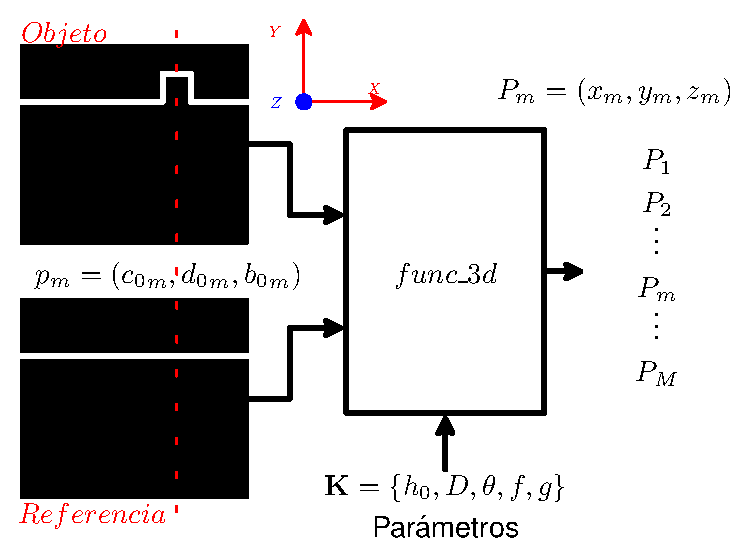
\includegraphics[width=\textwidth]{Diagrama3.eps}
         \caption{Diagrama de blocos.}
         \label{fig:blocos:sys}
     \end{subfigure}
     \hfill
     \begin{subfigure}[b]{0.425\textwidth}
         \centering
         \includegraphics[width=\textwidth]{Diagrama2.eps}
         \caption{Objeto em estudo.}
         \label{fig:blocos:obj}
     \end{subfigure}
\caption{Obtendo uma linha em 3D.}
\label{fig:blocos}
\end{figure}
Podemos ver todo este processo resumido na Figura \ref{fig:blocos:sys},
onde são extraídos $M$ pontos $p_m$ (em 2D) das imagens binarias 
e são convertidos em pontos $P_m$ (em 3D),
mediante a função $func\_3d()$ 
\begin{equation}
P \leftarrow func\_3d(p;\mathbf{K}),
\end{equation}
\begin{equation}
p=(c_0,d_0,b_0)\quad \xrightarrow[\mathbf{K}]{func\_3d} \quad P=(x,y,z),
\end{equation}
\begin{equation}
p_m=({c_0}_m,{d_0}_m,{b_0}_m)\quad \xrightarrow[\mathbf{K}]{func\_3d}\quad P_m=(x_m,y_m,z_m).
\end{equation}

Os pontos $p_m$ são extraídos um por cada coluna das imagens binarias,
e estão referenciados ao centro da imagem, é dizer os valores em $p_m$ podem ser positivos ou negativos.
A Figura \ref{fig:blocos:obj} mostra como são selecionados os valores $(c_0,d_0,b_0)$ para um ponto $p$,
que está ressaltado com um circulo vermelho na imagem. 
O centro da imagem está representado com um circulo azul.
O valor $d_0$ representa a distancia vertical de um ponto da linha de referencia ao centro da imagem,
o valor $c_0$ representa a distancia vertical de um ponto da linha do objeto à linha de referencia, e
o valor $b_0$   representa a distancia horizontal de um ponto da linha do objeto ao centro da imagem.

Os parâmetros do sistema $\mathbf{K}\equiv \{h_0,D,\theta,f,g\}$ são agrupado num vetor $\mathbf{K}$,
e estos valores são extraídos da geometria do sistema; 
por este motivo estes valores não mudam para todos os pontos $p_m$, $\forall~ 1\leq m \leq M$.
A Figura \ref{fig:setup1} mostra uma vista sagital da disposição do sistema,
onde as variáveis $h_0$, $D$, $\theta$, $f$ e $g$ são obtidas. 
Dado que a vista é sagital somente são mostradas aqui os valores $y$ e $z$
de um ponto $P=(x,y,z)$;
onde $z$ representa  altura do objeto e 
$y$ a distancia vertical da base do objeto em estudo ao ponto no plano de referencia a onde aponta a câmera;
este ponto é considerada a posição $(0,0,0)$ em 3D.
\begin{figure}[!h]
     \centering
         \includegraphics[width=0.7\textwidth]{Diagrama1.eps}
\caption{Vista sagital do sistema.}
\label{fig:setup1}
\end{figure}

A função $func\_3d()$ calcula a altura $z$ de um ponto mediante as
Equações (\ref{eq:setup1}) e (\ref{eq:setup2}),
\begin{equation}\label{eq:setup1}
z=\frac{
D~tg(\theta)
\left[
1+ ctg\left(\theta+atg\left(\frac{h_0}{d_0+c_0}\right)\right) ctg\left(\theta-atg\left(\frac{d_0}{h_0}\right)\right) 
\right]
}{
\left[1+ctg\left(\theta+atg\left(\frac{h_0}{d_0+c_0}\right)\right) ctg(\alpha)\right]
},
\end{equation}
\begin{equation}\label{eq:setup2}
ctg(\alpha)=\frac{D~tg(\theta)ctg\left(\theta-atg\left(\frac{d_0}{h_0}\right)\right)- f}{g}.
\end{equation}

O valor $y$ de um ponto analisado pode ser calculado mediante as
Equações (\ref{eq:setup3}) e (\ref{eq:setup2}),
\begin{equation}\label{eq:setup3}
y=D~tg(\theta)ctg\left(\theta-atg\left(\frac{d_0}{h_0}\right)\right)-D-z~ctg(\alpha).
\end{equation}

Para obter o valor $x$ são criadas as variáveis temporais $\gamma$ e $\beta$, como mostra 
a Figura \ref{fig:blocos2:sagital}.
Se geramos um plano com um angulo $\gamma$
obtemos uma vista onde a variável $x$ está evidente, como mostra a Figura \ref{fig:blocos2:plano}.
\begin{figure}[!h]
     \centering
     \begin{subfigure}[b]{0.475\textwidth}
         \centering
         \includegraphics[width=\textwidth]{Diagrama5.eps}
         \caption{Vista sagital do sistema.}
         \label{fig:blocos2:sagital}
     \end{subfigure}
     \hfill
     \begin{subfigure}[b]{0.475\textwidth}
         \centering
         \includegraphics[width=\textwidth]{Diagrama4.eps}
         \caption{Vista do plano com angulo $\gamma$.}
         \label{fig:blocos2:plano}
     \end{subfigure}
\caption{Detecção de cores.}
\label{fig:blocos2}
\end{figure}
Destas figuras concluímos que a variável $x$ pode ser obtida das Equações (\ref{eq:setup2:x}), 
 (\ref{eq:setup2:gamma}) e (\ref{eq:setup2:beta})
\begin{equation}\label{eq:setup2:x}
x=b_0\left(\frac{D~tg(\theta)-z}{h_0}\right)\left(\frac{csc\left({\gamma}\right) }{\sec\left(\beta\right)}\right),
\end{equation}
\begin{equation}\label{eq:setup2:gamma}
\gamma=\theta-\beta,
\end{equation}
\begin{equation}\label{eq:setup2:beta}
\beta=atg\left(\frac{c_0+d_0}{h_0}\right).
\end{equation}
\end{document}
